\documentclass[11pt, oneside]{article}   	
\usepackage[text={7in,9in},centering]{geometry}                		
\geometry{letterpaper}                   		
\usepackage[parfill]{parskip}    		
\usepackage{graphicx}						
\usepackage{amssymb}
\usepackage{float}
\restylefloat{figure}

\title{Simulating Virus and Host Coevolution Using Evolutionary Computation}
\author{Laura Colbran, Samuel Greaves, Liz Shank}
\date{}							

\begin{document}
\maketitle
\section{Introduction}
Bacteria and viruses both cause disease in humans ranging from the common cold to deadly epidemics such as bubonic plague. However, there are many more species of both that don't interact directly with humans. One example of this is those species of viruses that can also cause disease in bacteria. The specialized viruses that do this are called bacteriophages, and are essentially packets of genetic information (DNA or RNA) enclosed in a protein capsule. Virus genomes are streamlined, containing only the genes necessary to replicate themselves and produce their protein capsules. With such limited materials to hand, they have to infect bacteria in order to actually carry out their replication. Infection is accomplished by landing on the bacteria's outer membrane and injecting the viral information into the cytoplasm (Figure 1) (Todar, 2012).

\begin{figure}[H]
	\centering
	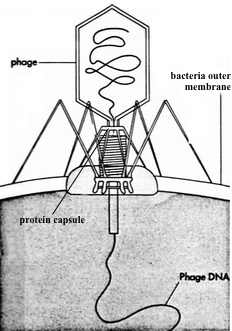
\includegraphics[width=0.42\textwidth]{figure1.png}
	\caption{A bacteriophage injecting its genome into a bacteria. The protein capsule both protects the 			genetic information while between hosts and pierces the membrane to allow injection. Adapted 			from Todar, 2012.}
\end{figure}

Once the genome has gained entry to the bacteria, the virus hijacks the machinery the host uses to replicate its own genome. In one mechanism of this, the virus incorporates its genome into the host genome, where it gets replicated and transported as the host cell reproduces. A different mechanism uses the host's ribosomes to synthesize proteins to promote virulence as well as new proteins to encapsulate new copies of the virus. Once there are many copies of the virus, they synthesize lysozyme, which breaks open the bacterial cell membrane, killing the host and allowing many new copies of the virus to escape and spread to nearby cells.

For the second mechanism, because the success of the virus means the death of the host, bacteria have evolved methods of resisting viruses. Coevolution has led to an arms race between viruses and bacteria, as they constantly find new ways to get around each other. This is especially evident in one model of virus-bacteria interaction known as gene-for-gene interaction. In these systems, the virus has a number of genes encoding virulence proteins that help it invade a cell and replicate its genome. Likewise, the bacteria has complementary resistance proteins that recognize and destroy the viral proteins. Through many generations, the viruses keep evolving new genes to get around the bacterial defenses, while the bacteria evolve to block resist the new genes. The progression of the genomes is cyclic, since selective pressure only acts on those loci where members of the bacteria population are still susceptible to the virus, and where the virus can still infect some bacteria. As the pressure lifts, specific resistance and virulence genes disappear from the population, since both host and parasite are prioritizing the genes most relevant to their interaction at that point in time (Person, 1959). The other extreme for virus-host interaction is the matching allele model, where virus genomes are disguised by being exactly identical to segments of the host genome. If the host's defenses cannot tell the difference between invasive genetic information and their own, then the virus can successfully infect the cell. These two models are ends of a continuum of interaction; in mature, most interactions are some mixture of the two systems (Agrawal and Lively, 2002).

One interesting side-effect of this arms race is the relatively elevated mutation rate in many bacteria populations. In 2007, Pal et al. used a mixture of techniques to demonstrate that it was specifically coevolution with viruses that drove the increased mutation rate in susceptible bacteria. The mutation rate was mostly increased over time due to deleterious mutations in mismatch-repair genes, which code for proofreading proteins that normally check new copies of the bacterial genome for mutations and correct them. Without functioning mismatch-repair proteins, mutations are much more likely to passed on without being fixed. One of the tools Pal et al. used in their research was a genetic algorithm that simulated host-virus interactions, which they used specifically to model how mutation rates evolved over time. Their simulation behaved similarly to the predictions of the gene-for-gene model, with host mutation rate plateauing at the maximum allowed, while the frequencies individual genomes fluctuate over time as the selection pressure shifts in response to viral evolution (Figure 2) (Pal et al., 2007).

For our project, we attempted to replicate the simulation run by Pal et al., using a coevolution genetic algorithm. We based the representation of populations and fitness functions on those detailed by that paper. Unlike most GAs, we did not use crossover to introduce variability, because reproduction done in our model system is asexual, meaning there is only one parent for each child, and therefore no opportunity to undergo crossover. Besides complete replication, we also made some alterations to increase the similarity of our simulation to how the bacteria-virus system operates in nature. 

\begin{figure}[H]
	\centering
	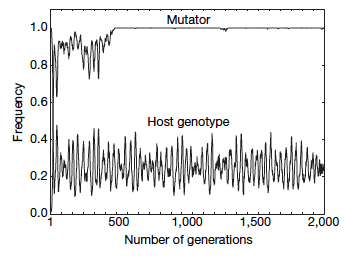
\includegraphics[width=0.75\textwidth]{figure2.png}
	\caption{Frequencies over time of a mutator gene that increases mutation rate 100-fold in the host 			population and one particular host genotype (Pal et al. 2007).}
\end{figure}

\section{Coevolutionary Genetic Algorithm}
Viruses and hosts are divided into two populations, with individual genomes being represented by ArrayLists of bit arrays. Both types of genomes have indices for interaction models and mutators, while viruses also have a set of virulence genes and bacteria have a set of resistance genes and one of viability genes (Table 1). The interaction model is either the gene-for-gene model, where the resistance/virulence bits represent genes, or the matching-allele model, where they represent a recognition sequence. In the former, viruses are able to infect if they have a virulence gene for which the bacteria doesn't have the corresponding resistance gene. In the latter, the virus can infect if its virulence sequence exactly matches the bacterial sequence. The mutator in both is switched off by default, but can mutate to increase to mutation rate of carriers by 100-fold. In bacteria, the viability genes serve as a trade-off for increased mutation rate. They can mutate to be deleterious, decreasing fitness, and an increased mutation rate makes that change more likely to occur. Any aspect of each genome can undergo mutation at a rate constant for both populations, except the individuals with mutators switched on. 

\begin{table}[H]
	\begin{center}
	 \begin{tabular}{||c c c c c||} 
	 \hline
	Individual & Interaction Model & Mutator & Resistance/Virulence & Viability\\ 
	& 1 bit & 1 bit & n bits & m bits\\
	 \hline\hline
 	Host & yes & yes & yes & yes\\
	 \hline
 	Virus & yes & yes & yes & no\\
	 \hline
	\end{tabular}
	\caption{Representation of Virus and Host Individuals. Both are ArrayLists of Arrays.}
	\label{table:1}
	\end{center}
\end{table}

Fitness for each virus is a function of the number of virulence genes in its genome, multiplied by the number of hosts in the current population it is capable of infecting:

\begin{equation}
W_{Pij} = (1-a\cdot p)^v\cdot N,
\end{equation}
where $v$ is the number of virulence genes, and N is the number of potential hosts. There is also a cost of virulence, mimicking a trade-off with prioritizing virulence over other genes, represented by $p$. $a$ is the bit representing the interaction model, which is 1 for the gene-for-gene model. For the matching-allele model, counting virulence and resistance genes is irrelevant, so that term equals zero.

The host's equation is more complicated, as it takes into account resistance, viability genes, and the fitness of any viruses infecting it. Fitness for host $i$ with $n$ deleterious mutations infected by virus $j$ is:
\begin{equation}
W_{H}(i,n) = (1-s_{v})^n(1-a\cdot c)^z(1-s\cdot W_{Pij}),
\end{equation}

where $s_{v}$ is the effect of each deleterious mutation, $c$ is the cost of each resistance allele, $z$ is the number of resistance alleles, $s$ is maximum virulence of the virus, and $W_{Pij}$ is the fitness of virus $j$ on host $i$. Total fitness for each host is $\sum W_{H}(i,n)$ for all viruses able to infect it. 

These fitness functions work with the interaction models to operate as a version of fitness-proportional selection (Figure 3). Viruses interact with a sample of the bacterial population, and fitnesses are evaluated before reproduction. Both viruses and bacteria undergo asexual reproduction, and have the potential to make many children. How fit an individual is determines what proportion of its maximum potential children actually get created. These clonal children undergo mutation at the rate dictated by their genome and the systemic mutation rate. Crossover does not occur, as each child has only one parent. Individuals die after reproducing and are removed from the population. The populations are allowed to vary, within certain limits analogous to a carrying capacity. If a population overshoots the limit, individuals are culled in a fitness-proportional manner, with the least fit individuals being more likely to be removed. We used a phylogenetic tree to track the progress of 'families' of individuals.

\begin{figure}[H]
	\centering
	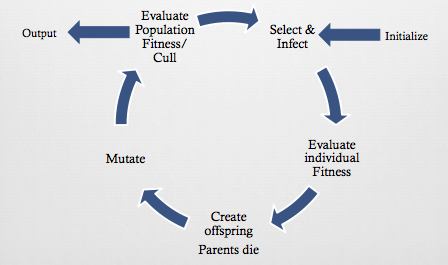
\includegraphics[width=0.7\textwidth]{flowchart.png}
	\caption{Flow chart diagramming what happens in each generation of the algorithm.}
\end{figure}

\section{Results of Simulation}
- graph demonstrating duplication of results (so comparison is valid!)
\\- what happens if we let viruses evolve frequent mutation?
\\- gradient of mutation rates?
\\- bacterial sampling methods
\\- evolving interaction models

\section{Discussion}
What was hard? What are some new results/what might they imply biologically? What are some new directions to try?

- interpreting their methods was interesting-- published for biologists! They didn't plan for people caring so much about their specific algorithm. 

\section{Works Cited}
Agrawal, A. and C.M. Lively. 2002. Infection genetics: gene-for-gene versus matching-alleles models and \\\-\hspace{0.75cm} all points in between. Evolutionary Ecology Research. 4: 79-90.

Pal, C., M.D. Marcia, A. Oliver, I. Schachar, and A. Buckling. 2007. Coevolution with viruses drives the \\\-\hspace{0.75cm} evolution of bacterial mutation rates. Nature Letters. 450: 1079-1081.

Person, C. 1959. Gene-for-gene relationships in host:parasite systems. Canadian Journal of Botany. 37: \\\-\hspace{0.75cm} 1101- 1130.

Todar, K. 2012. Bacteriophage. Online Textbook of Bacteriology. Accessed 6.4.2015.\\\-\hspace{0.75cm} http://textbookofbacteriology.net/phage.html

\end{document}  